%!TEX root = ../../main.tex
\chapter{Material und Methoden}
\section{Datensatz: \ac{BraTS}}
Der \ac{BraTS} Datensatz ist ein öffentlich verfügbarer Datensatz, der für die Entwicklung und Evaluierung von \glspl{Modell} für die Segmentierung von Gehirntumoren verwendet wird. Er wurde von der Radiological Society of North America in Partnerschaft mit der American Society of Neuroradiology(ASNR) und Medical Image Computing and Computer Assisted Interventions(MICCAI) erstellt und besteht aus über tausend \ac{MRT} Bildern von verschiedenen Patienten mit Hirntumoren. \cite[vgl.][]{RSNABrainTumor2021}

\subsection{Beschreibung}
\label{subsec:Beschreibung}
Der Datensatz enthält multi-institutionellen und multi-parametrischen \ac{MRT} Scans (mpMRT), die unter klinischen Standardbedingungen mit unterschiedlichen Geräten und Protokollen aufgenommen wurden. ``Multi-institutionell'', bezieht sich darauf, dass die Daten für den Datensatz von mehreren medizinischen Einrichtungen bereitgestellt und zusammengeführt wurden. ``Multi-parametrisch'' bedeutet, dass der Datensatz mehrere Parameter bzw. Merkmale enthält, welche für die Segmentierung der Hirntumore verwendet werden können. \\
Für die Aufgabe der Segmentierung wurden alle Gehirntumore mit den führenden BraTS-Algorithmen segmentiert und anschließend von freiwilligen Neuroradiologie Experten mit unterschiedlicher Erfahrung nochmals verfeinert. Für die manuellen Beschriftung der Daten wurde ein strenges Protokoll eingehalten, um einheitliche Daten zu erhalten. Abschließend wurden die manuell verfeinerten Bilder von zertifizierten und erfahrenen Neuro-Radiologen mit mehr als 15 Jahren Erfahrung in dieser Tätigkeit bestätigt. 
Die beschrifteten Tumor-Regionen basieren auf den VASARI-Merkmalen\footnote{VASARI-Merkmale(Visually Accesable Rembrandt Images) sind ein System für die konsistente Beschreibung von Gliomen (Tumoren) mithilfe definierter visueller Merkmale \cite[vgl.][]{Nam2021}}, welche für einen geschulten Radiologen sichtbar sind. Diese Merkmale umfassen den mit Gadolinium anreichernden Tumor (Kennzeichnung 4), das peritumorale ödematöse/invasive Gewebe (Kennzeichnung 2) und den nekrotischen Tumorkern (Kennzeichnung 1). \cite[vgl.][]{Baid2021}
\begin{figure}[ht]
	\centering
	\begin{subfigure}[b]{0.4\textwidth}
		\centering
		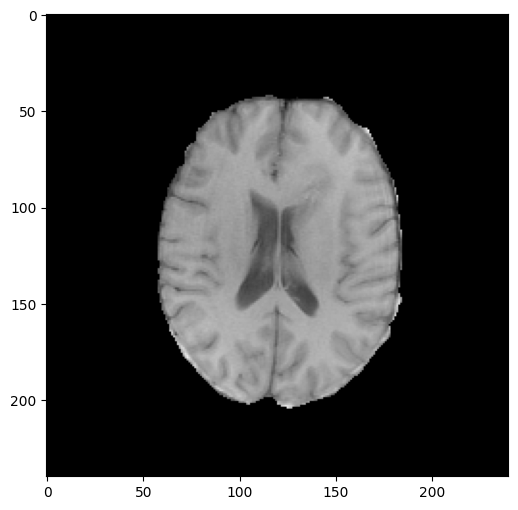
\includegraphics[width=\linewidth]{mrt_t1.png}
		\caption{T1-Gewichtung}
		\label{fig:t1}
	\end{subfigure}
	\hfill
	\begin{subfigure}[b]{0.4\textwidth}
		\centering
		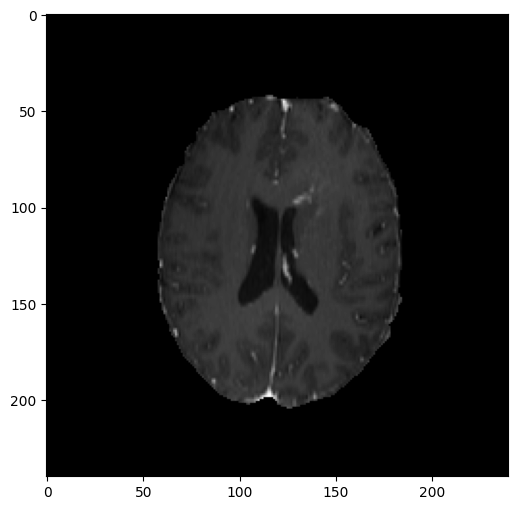
\includegraphics[width=\linewidth]{mrt_t1ce.png}
		\caption{kontrastverstärkte T1-Gewichtung}
		\label{fig:t1ce}
	\end{subfigure}
	\vskip\baselineskip
	\begin{subfigure}[b]{0.4\textwidth}
		\centering
		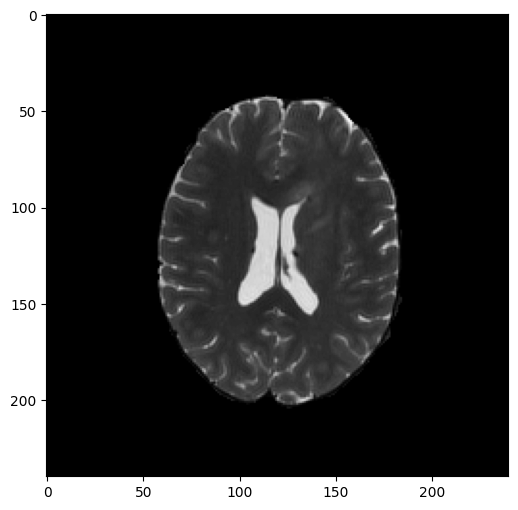
\includegraphics[width=\linewidth]{mrt_t2.png}
		\caption{T2-Gewichtung}
		\label{fig:t2}
	\end{subfigure}
	\hfill
	\begin{subfigure}[b]{0.4\textwidth}
		\centering
		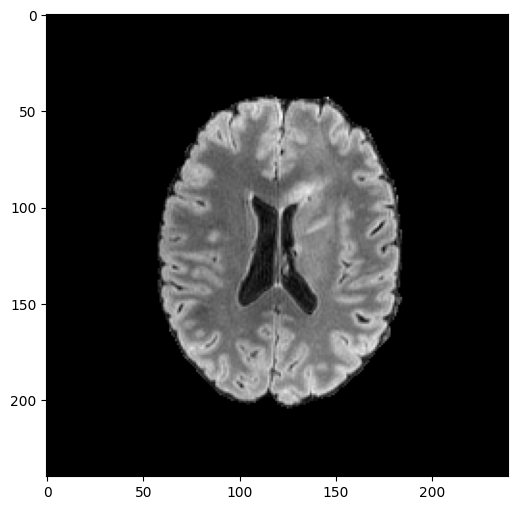
\includegraphics[width=\linewidth]{mrt_flair.png}
		\caption{Flair-Gewichtung}
		\label{fig:flair}
	\end{subfigure}
	\caption{Die vier Modalitäten im Datensatz}
	\label{fig:mrt_scans}
\end{figure} 

Der Datensatz enthält 1251 Einträgen, jeder Eintrag besteht aus einer T1-, kontrastverstärkte T1-, T2- und Flair-Gewichtung (siehe Abb. \ref{fig:mrt_scans}) sowie einer fertigen Segmentierung des Hirntumors. Die Dateien selbst sind im NIfTI-Dateiformat, was für ''Neuroimaging Informatics Technology Initiative`` steht und ein gängiges Format für medizinische Bilddaten ist. Das Dateiformat enthält die 3D-Volumendaten, welche aus mehreren Schichten von Bildern bestehen. Jedes Voxel, ein 3D-Bildpunkt, enthält einen numerischen Wert, der das Signal bzw. den Kontrast widerspiegelt. Zusätzlich enthält das NIfTI-Dateiformat Metadaten, wie die räumliche Orientierung, Bildgröße,Raumkoordinaten und weitere Metadaten. \cite[][]{NIfTI} Die Bilder liegen in einer Größe von 150x240x240 Pixeln vor, dies entspricht wie bereits erwähnt den 3D-Volumendaten, welche in 150 Schichten aufgeteilt wurden, wobei jede Schicht ein Bild in der Größe von 240x240 Pixeln entspricht.


\subsection{Vorverarbeitung}
Die Vorverarbeitung der Daten ist ein wichtiger Schritt, damit sich die Qualität und Effektivität des Trainings von einem Neuronalen Netz verbessern. Der bereitgestellte Datensatz wurde bereits einer Standard Vorverarbeitung (engl.: Pre-Processing) unterzogen. Zunächst wurden die Daten vom DICOM-Dateiformat in das NIfTI-Dateiformat konvertiert, was zur einfacheren Handhabung der Daten dient. Ebenfalls wurde eine Anpassung auf gleiche anatomische Vorlage und isotrope Auflösung getätigt. Abschließend wurde  das Skull-Stripping\footnote{Skull-Stripping ist der Prozess des Entfernens von Schädel und anderen nicht auf das Hirn bezogenen Strukturen vom Bild. \cite[vgl.][]{SwiebockaWiek2016}} durchgeführt um irrelevante Strukturen zu entfernen. \cite[vgl.][]{Baid2021}

\paragraph{Normalisierung}
Nach diesen Schritten sind die Daten noch nicht für das Training eines Neuronalen Netzes geeignet. Die Daten müssen zunächst normalisiert werden, dies kann auf zwei Wegen geschehen. Entweder die Werte werden auf einen Bereich von 0 bis 1 skaliert oder man verwendet die Z-Standardisierung. Bei einer einfachen Skalierung der Werte wird folgende Gleichung verwendet
\begin{equation}
	f(x)=\frac{x - min(x)}{max(x) - min(x)}
\end{equation}

Dies führt zwar zu einer Vereinheitlichung der Werte, jedoch ist die Verteilung der Merkmale im Bild so nicht normiert. Für dieses Vorhaben verwendet man die Z-Standardisierung, welche den Mittelwert der Daten auf 0 und die Standardabweichung auf 1 bringt. Es wird verhindert, dass bestimmte Merkmale dominant werden, im Vergleich zu anderen. Zudem wird die Genauigkeit des \glspl{Modell} erhöht.\cite[vgl.][]{Goodfellow2016} Die gleich für die Z-Standardisierung lautet
\begin{equation}
	f(x)=\frac{x - \mu_x}{\sigma_x}
\end{equation}
wobei $\mu_x$ der Mittelwert und $\sigma_x$ die Standardabweichung des Datensatzes ist. Diese Werte müssen vorab berechnet werden, in dem der Mittelwert und die Standardabweichung von jedem Bild berechnet wird, anschließend aufsummiert und durch die Anzahl der Bilder geteilt wird
\begin{equation}
	\begin{aligned}
		\mu &= \frac{1}{n}\sum_{i=1}^{n}x_i \\ \\
		\sigma &= \sqrt{\frac{1}{n}\sum_{i=1}^{n}(x_i - \mu)^2}
	\end{aligned}
\end{equation}
wobei $n$ die Anzahl der Bilder und $x_i$ ein Bild des Datensatzes ist.

\paragraph{Data Augmentation} 
Im medizinischen Bereich sind die Bilddaten oft begrenzt, weshalb sich das Training eines Neuronalen Netzes dadurch erschwert. Eine Methode dem entgegen zu wirken ist die Data Augmentation, bei welcher die Diversität des Trainingsdatensatzes erhöht wird. Verschiedene Augmentierungen sind Bildbearbeitungsmethoden wie das Rotieren, Skalieren, Ausschneiden oder auch Spiegeln eines Bildes. Es ist wichtig darauf zu achten, dass alle Augmentierungen sowohl auf die Eingangsbilder, als auch auf die dazugehörigen Segmentierungen angewendet werden, da das Neuronale Netz sonst falsche Masken für die Eingaben erlernt. \cite[vgl.][]{Shorten2019}

\paragraph{3D-Bild zu 2D-Bilder} 
Die Daten liegen als 3D-Bilddaten vor, jedoch ist die Anzahl der Daten mit 1251 Bildern eher gering. Um mehr Bilder aus den vorhandenen Daten zu bekommen, werden die 3D-Bilder in einzelne 2D-Bilder geschnitten. Wie bereits in Abschnitt \ref{subsec:Beschreibung} erwähnt, besteht ein 3D-Bild aus 150 geschichteten Bildern mit der Größe von 240x240 Pixeln. Jede einzelne Schicht wird als Separates Bild abgespeichert, um so die Anzahl der Daten zu erhöhen, so entstehen aus einem 3D-Bild 150 einzelne 2D-Bilder. Es wird jedoch nicht nur die Anzahl der Daten erhöht, sondern auch die Geschwindigkeit der Berechnungen, da dies im zweidimensionale weniger Rechenleistung und Speicher benötigt. Die Konvertierung von 3D- in 2D-Bilder bringt aber auch Nachteile mit sich, wie der Verlust des räumlichen Zusammenhangs zwischen den einzelnen Schichten. \cite[vgl.][]{Stevens2020}

\paragraph{Größen Skalierung}
\label{paragraph:GrößenSkalierung}
Bei manchen Neuronalen Netzen, kann die Größe des Bildes eine Rolle spielen. Es gibt Architekturen, bei denen die Bildgröße beliebig sein kann, oder das Eingabebild eine bestimmte Größe vorweisen muss, damit es verarbeitet werden kann. \\
Die Architektur welche für die Segmentierung der Gehirntumore verwendet wird, ist ein U-Net und wird in Kapitel \ref{sec:Modellarchitektur} genauer beschrieben. Aufgrund der besonderen Architektur des UNets, müssen die Bilder eine bestimmte Größe haben. Der Grund für die spezifische Eingabegröße liegt in der Architektur des UNets, genauer gesagt durch die Down- und Upsampling Pfade. Die Größe des Bildes, wird schrittweise durch Konvolution und Max-Pooling Schichten auf der einen Seite reduziert und auf der anderen Seite wieder vergrößert. \\
Aufgrund des Designs des U-Net muss die Größe der Bilder ein Vielfaches von der Anzahl der Downsampling-Schichten sein. Die Größe der Bilder wird durch die Gegebenheiten definiert durch $2^N$, wobei $N$ die Anzahl der Downsampling-Schichten ist. Sei $N=4$, so muss die Eingabegröße der Bilder ein vielfaches von $2^4=16$ sein. Ist nicht die richtige Größe gegeben, so kann es zur Inkonsistenz der Größen kommen, was wiederum die Leistung des \gls{Modell}s beeinflusst. \cite[vgl.][]{Ronneberger2015}

Um die Bilder in eine geeignete Größe zu bringen werden sie von der Mitte ausgehend nach außen hin ausgeschnitten. Die Größe des Bildausschnittes beträgt im Grunde 128x128 Pixel. Es kommt jedoch vor, dass Teile des Gehirns abgeschnitten werden (siehe Abb. \ref{fig:GrößeOhnePuffer}), weshalb noch ein Puffer von 60 Pixeln je Rand hinzugefügt wurde. Nach Hinzufügen des Puffers ist das Bild nicht mehr in einer geeigneten Größe und wird abschließend auf eine Größe von 128x128 Pixeln skaliert (siehe Abb. \ref{fig:GrößePuffer}).
\begin{figure}[ht]
	\centering
	\begin{subfigure}[b]{0.4\textwidth}
		\centering
		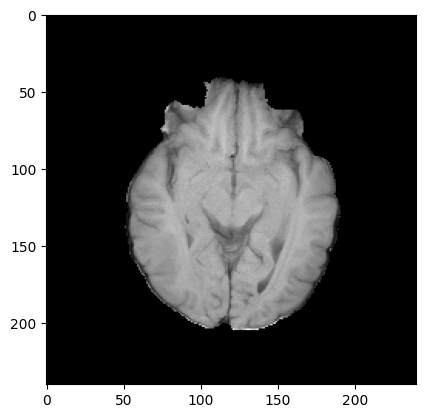
\includegraphics[width=\linewidth]{img_size_original.png}
		\caption{Original Bild}
		\label{fig:GrößeOrg}
	\end{subfigure}
\vfil
	\begin{subfigure}[b]{0.4\linewidth}
		\centering
		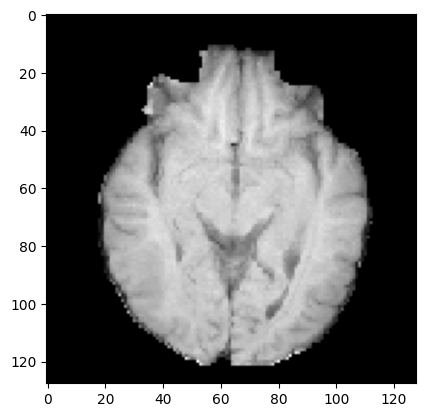
\includegraphics[width=\textwidth]{img_size_crop_puffer.png}
		\caption{Ausschnitt mit Puffer}
		\label{fig:GrößePuffer}
	\end{subfigure}
\hfil
	\begin{subfigure}[b]{0.4\linewidth}
		\centering
		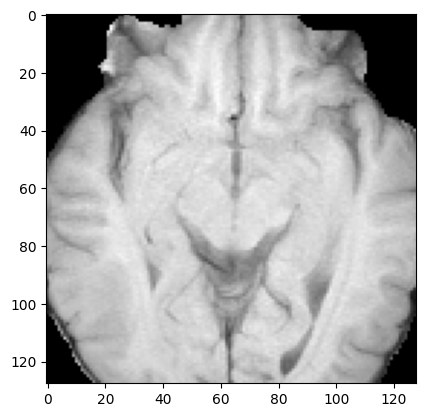
\includegraphics[width=\textwidth]{img_size_crop.png}
		\caption{Ausschnitt ohne Puffer}
		\label{fig:GrößeOhnePuffer}
	\end{subfigure}
	\caption{Orginal Bild (T1-Gewichtung) im Vergleich zum Ausschnitt mit und ohne Puffer.}
\end{figure} 


\subsection{Aufteilung}
Es ist wichtig den Datensatz in verschiedene Teile aufzuteilen, damit die Entwicklung eines Modells gelingt. Der Datensatz wird dafür in einen Trainings-, Validerungs- und Testdatensatz aufgeteilt. Diese verschiedenen Datensätze ermöglichen es die Leistung und die Generalisierungsfähigkeit des \gls{Modell}s zu beurteilen. \\
Der Trainingsdatensatz wird verwendet, um das Modell zu trainieren, indem es die internen Modellparameter anhand der Eingabedaten und den dazugehörigen Beschriftungen anpasst. Je größer der Trainingsdatensatz ist, desto besser kann das \gls{Modell} generalisieren, da es viele Daten mit unterschiedlichen Merkmalen lernt. \\
Um die Leistung des \gls{Modell}s während des Trainings zu beurteilen wird der Validierungsdatensatz verwendet. Anhand der Ergebnisse auf dem Validierungsdatensatz, werden die Hyperparameter des \gls{Modell}s angepasst. Es ist wichtig darauf zu achten, dass dieser Datensatz keine Überschneidungen mit dem Trainingsdatensatz hat, da es sonst zu falschen Ergebnissen kommt. \cite[vgl.][]{Weidman2020}
Möchte man das Modell abschließend nochmals evaluieren, so kommt oft ein Testdatensatz zum Einsatz, den das \gls{Modell} noch nie vorher gesehen hat. Nach dem das Training mit dem Trainings- und Validierungsdatensatz abgeschlossen ist, kann der Testdatensatz herangezogen werden, um die finale Leistung des \glspl{Modell} zu beurteilen.